\chapter{Introduction: Human-Robot interaction and Knowledge}
\label{chapter|introduction}


This shift requires ``awareness'' of humans.

To make informed decision, the robot needs knowledge about the \emph{tasks},
the \emph{environment}, the \emph{situational context}.
%%%%%%%%%%%%%%%%%%%%%%%%%%%%%%%%%%%%%%%%%%%%%%%%%%%%%%%%%%%%%%%%%%%%%%%%%%%%%%%

List of recent successful \& highly visible robot experiments in human environment:
\begin{itemize}
    \item Amener une bierre avec le PR2 (WG)
    \item Sandwiches/popcorn at TUM
    \item expe avec Nao
\end{itemize}

Service robotics is leaving the realm of Sci-Fi, dreams and fanstasms to become
a reality. \fxwarning{find references of predictions "when robots are in our
homes}. 

Robotics is moving from technological demos to real world coworkers/companions.


Decision making on the robot can not anymore rely on a single or a few
modalities of interaction.

The perceptual layer has moved up from traditional sensing modalities (camera
images, laser scans) to synthetic sensing devices like the Kinect-based human
tracker, face recognition or SLAM-based localization.

Perceiving and understanding the environment is now mainly a matter of
rebuilding an internal, amodal, model of the environment with to interleaved
facets: a continuous, geometric world and a discrete, symbolic world.

Because we are now interested in having the robot to not live anymore in
isolation, but on contrary, in interaction with other intelligent agents, we
want to endow our systems with \emph{agency} and \emph{social skills}. This
implies that the robot is able not only to represent inanimate objects but also
other intelligences, other minds. And not only represent them, but also
interact with them, which require communication skills, ability to take
perspectives and a theory of mind.

Note that our robot comes to life in a connected world. It has to interact with
other agents that may physically exist or may be equally well disembodied.

Figure~\ref{fig|congitive-robots} proposes an organization of research fields
and projects in robotics along two dimensions, the level of social skills, and
the level of agency (the ability to \emph{act in the world}).

\begin{figure}
    \centering
    
\includegraphics[width=0.7\columnwidth]{intro/social_skills.pdf}
    \caption{Towards the cognitive robot}
    \label{fig|cognitive-robots}
\end{figure}


%%%%%%%%%%%%%%%%%%%%%%%%%%%%%%%%%%%%%%%%%%%%%%%%%%%%%%%%%%%%%%%%%%%%%%%%%%%%%%%
%%%%%%%%%%%%%%%%%%%%%%%%%%%%%%%%%%%%%%%%%%%%%%%%%%%%%%%%%%%%%%%%%%%%%%%%%%%%%%%
%%%%%%%%%%%%%%%%%%%%%%%%%%%%%%%%%%%%%%%%%%%%%%%%%%%%%%%%%%%%%%%%%%%%%%%%%%%%%%%

\section{The general context of Human-Robot interaction in this work}
\label{sect|general-context}

Interaction for \emph{joint action} in a \emph{situated} environment.

%%%%%%%%%%%%%%%%%%%%%%%%%%%%%%%%%%%%%%%%%%%%%%%%%%%%%%%%%%%%%%%%%%%%%%%%%%%%%%%
%%%%%%%%%%%%%%%%%%%%%%%%%%%%%%%%%%%%%%%%%%%%%%%%%%%%%%%%%%%%%%%%%%%%%%%%%%%%%%%
%%%%%%%%%%%%%%%%%%%%%%%%%%%%%%%%%%%%%%%%%%%%%%%%%%%%%%%%%%%%%%%%%%%%%%%%%%%%%%%

\section{A Prototypical Scenario}
\label{sect|scenario}

\begin{figure*}
	\centering
	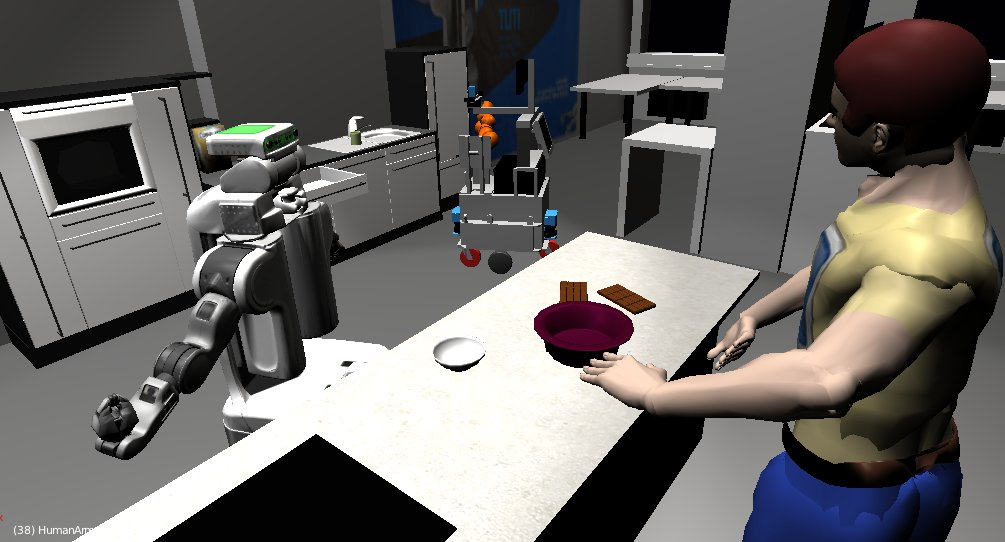
\includegraphics[width=0.9\textwidth]{intro/brownie_scenario.jpg}
	\caption{A representation of the scenario, in the MORSE simulator}
	\label{fig|scenario}
\end{figure*}

In order to illustrate what we consider to be the required features of a
knowledge representation system for robotics, we introduce in this section a
demonstration scenario.

While devising a scenario inevitably constraints the breadth of abilities we
examine, we insist on the fact that our main purpose here is to ground into a
real case the set of representational features we consider as desirable.  We
will \emph{not} evaluate any of the systems we survey in this article by
judging their applicability to this particular scenario.

We entitle our scenario ``the Brownie scenario'' (Fig.~\ref{fig|scenario}).

Robi and Roba are two service robots. They are considered to be able to freely
move and pick objects, but they are not expected to have the exact same
hardware and softwares architectures, and specially, they are not expected to
have the same knowledge representation system. These robots cooperate with a
human in a kitchen environment.

The main task of the scenario is the joint realization of a brownie, initiated
by the human injunction ``Let's make a brownie for tonight!''.

The scenario is successful if the task is achieved (the brownie is baked) and:

\begin{itemize} 

	\item it took less time that it would have require for the human alone, 

	\item it didn't require a heavier cognitive involvement from the human that
	what would have been required without the robots' help.  

\end{itemize}

We voluntarily do not detail the subtasks of the scenario, neither we define
how they are shared amongst agents. In our analysis we focus on the general,
\textit{a priori} representational needs of the scenario.

A ``first-order'' analysis of this task leads to a first partition of the
required representation abilities:

\begin{enumerate}

	\item Representation abilities related to the execution of a complex
	spatio-temporal task,

	\item Representation abilities related to cooperation with other agents.

\end{enumerate}

% Representation of a complex task
We can further refine these categories: to prepare and bake a brownie, the
robot first needs to make sense of the very term \emph{brownie}: what is it?
what is it used for? what is it made of? etc. We call this knowledge
\emph{common-sense knowledge} and the robot must be able not only to represent
it, but also to have some kind of access to it (for instance through a initial
set of facts that are made available at startup, or via access to a Web-based
knowledge base like Wikipedia, etc.)

Bound to the action \emph{make}, this should lead the robot to build and
represent a \emph{context}: we are in a scenario involving cooking. Actions
related to cooking often take place in the kitchen, cooking requires ingredients, 
utensils and a procedure that may be provided by a recipe, etc.

This last sentence implies several other features for our knowledge
representation system: ``cooking often takes place in the kitchen'' implies
that representation of both uncertainty and likelihood is desirable. The fact
that cooking is associated to a place further implies that the system models
locations and is able to attach \emph{thematic relations} to concept
(here, the likely location of the cooking action).

``cooking requires ingredients that may be provided by a recipe'' hints about a
very common feature available in most knowledge representation systems:
\emph{reasoning}. The robot \emph{infers} that cooking may require a recipe
since a list of ingredients is a pre-requisite of the cooking action, and a
recipe may provide such a list. If we omit the ``may'', this is a typical
example of first-order logic reasoning. Many other reasoning techniques exist
(including probabilistic ones -- ones able to deal with the ``may''), we shall
illustrate some of them later in this scenario.

We mentioned that a recipe often provides a procedure (or a \emph{plan}). The robot
should be able to store this plan in a way that allow later execution.  The
plan is likely to contain \emph{spatio-temporal constraints} (like ``put
the brownie in the oven for 20 min'') that must as well be appropriately
represented.

To make decision, a robot may also want to \emph{predict} the state of the world
after some action (``if I leave the cake 2h in the oven, it will be burned'').
Such ability to project itself in future or, generally speaking, in other
possible state of the world is related to several cognitive ability and
reasoning techniques: \emph{planning}, \emph{representation of possible worlds}
and \emph{non-monotonic reasoning}, in addition to common-sense knowledge and
\emph{physics-based reasoning}.

Procedures are in addition often \emph{underspecified}: we can expect the recipe
to provide a cooking duration, but we usually do not expect the recipe to tell
us to first open the oven door, and then put the cake into it, since it is
self-evident that the door must first be opened to put the cake in the oven.
Such underspecification should be detectable, representable, and ideally
completable by the knowledge representation system\footnote{Note that we do not
assume here the {\it knowledge representation system} to be a single software
component: it may well be the result of the aggregation of several modules
working together}.

% Representation feature that enable cooperation
Then, we want our three agents to cooperate. This, in turn, leads to another
set of cognitive abilities.

Cooperation in our scenario can intervene at many places. For instance, an
agent may want to inform another one about the number of eggs that are
necessary for the brownie. This \emph{helping} behaviour makes sense only if
the first agent knows that the recipient agent both needs the information but
does not know it. This in turn requires the robot to be able to model the
knowledge of the other agents: to think \emph{from the perspective} of another
agent (this idea is related to the so-called Theory of Mind~\cite{...}).

Ability to communicate is one important pre-requisite to collaboration.
Communication in general~\cite{Jakobson} requires the addresser and the
addressee to share a common interpretative framework (shared common-sense
knowledge -- or cultural background -- and a shared context). In our scenario,
the agents are working in a kitchen. This element of context does not however
suffice if, for example, an agent asks another agent to ``give {[him]} the
bowl''. Besides the symbol ``bowl'', which physical entity are we actually
talking about? If we want to act on the world, this so-called \emph{grounding}
operation is essential, and may be tightly bound to the underlying knowledge
representation system. Note that grounding usually denotes the {\it top-down}
operation: from the symbol to the percept. It is however commonly bundled with
the converse operation, that retrieve (or create) symbols from perception.

A related ability is called \emph{pre-supposition accomodation}: if one of the
agent moves behind another one, with the brownie dough in its arm, and says
``be careful, I'm behind you!'', we want the first agent to be able to
represent both symbolically and geometrically (because, for instance, if the
agent want to move, it must take into account the new obstacle) something that
was not directly perceived. A knowledge representation system may be able to
provide structures to represent and reason about such cases.

Also central to cooperation are the notions of \emph{joint
intentions} and \emph{joint goals}~\cite{Tomasello2005, Bratman2009}: to help
the human during the cooking session, the robots need to track how far
they are into the recipe, what is the next step the human is likely to go for,
how task are currently split between agents, what action is currently
blocking the procedure, etc. This knowledge should let the robot identify the
intentions of other agents and create accordingly joint goals. Hence, a
knowledge representation system aiming at dealing with cooperative behaviours
is likely to have goal management structures taking explicitly into account
other agents' actions and goals.

In order to effectively share tasks, the robot must also know what it is
capable of: \emph{capability introspection} (both in term of general capability
and of immediate ability) is thus often desirable. More general introspection
(like the ability to tell ``who I am'' or ``what do I think of'' does not
appear to be necessary in our scenario. This may however enrich the human-robot
interaction.

Last but not least, our scenario assumes implicitly \emph{natural interaction}
between humans and robots (as showed by the casual style of the
order ``Let's make a brownie!''). While natural language processing {\it
per-se} is usually out of the scope of a knowledge representation system, we
may want to be sure these systems may successfully interoperate, \ie that the
knowledge representation system provides efficient support to the natural
language processing module (for instance by adopting models and vocabulary that
are both well suited for machine processing and remain as close as possible to
the humans own structures and vocabulary).

%%%%%%%%%%%%%%%%%%%%%%%%%%%%%%%%%%%%%%%%%%%%%%%%%%%%%%%%%%%%%%%%%%%%%%%%%%%%%%%
%%%%%%%%%%%%%%%%%%%%%%%%%%%%%%%%%%%%%%%%%%%%%%%%%%%%%%%%%%%%%%%%%%%%%%%%%%%%%%%
%%%%%%%%%%%%%%%%%%%%%%%%%%%%%%%%%%%%%%%%%%%%%%%%%%%%%%%%%%%%%%%%%%%%%%%%%%%%%%%


\section{What are the challenges?}
\label{sect|scenario-challenges}

Those two broad targets should lead to two improvements for human-robot
interaction:


\begin{itemize}
	\item to loosen the constraints on symbolic modelling of the robot
	environment by providing more expressive representation system than
	classical databases or fact repositories,

	\item to improve human-robot interaction by explicitely providing to the
	machine an interpretation frame, at least partially shared with the human.

\end{itemize}


\fxnote{Put focus on knowledge related challenge => focus on questions that need to be
answered}
\fxnote{Show what is difficult in the scenario, and why this requires research.}

\subsection{Specific requirements of human-robot interaction}
\label{sect|pecularities-krs-for-hri}

Pecularities on knowledge representation required by HRI, in the frame of the
general context defined in section~\ref{sect|general-context}:

\subsubsection{Human communication}

\begin{figure}%[!ht]
\centering
  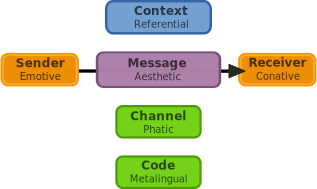
\includegraphics[width=0.6\linewidth]{communication/jakobson_communication_model.pdf}
  \caption{The \emph{Communication Model}, as proposed by Jakobson. In bold
  characters are the \emph{communication dimensions}, in italics, the
  corresponding \emph{communication functions}.}
  \label{fig|jakobson_communication_model}
\end{figure}

\subsubsection{Perspective-Taking, False Beliefs, Theory of Mind}

\fxnote{Present here Sally and Ann}

\subsubsection{and also...}

\begin{itemize}
	\item Ability to talk about concepts that are not immediately perceived by
	the robot


	\item \fxerror{TBD: absence of knowledge representation} Ability to
	represent that an agent knows something about something else, even if we do
	not know \emph{what}.

\end{itemize}

\subsection{Targeted applications/experiments}
\label{sect|targeted-applications-experiments}


The operational targets are two-fold:

\begin{inparaenum}[\itshape a\upshape)]

	\item determine, for a abstract/theoritical/general point of view, how and
	why a cognitive architecture could contribute to these aims; and

	\item implement it.

\end{inparaenum}

\begin{itemize}
	\item \textbf{Categorization}: \emph{Odd One Out}-style experiment,
	\item \textbf{Dialogue}: Grounded dialogue,
	\item \textbf{Introspection verbalization}: Integration dialogue/planing, verbalization of plans,
	\fxerror{TDB: integration dialogue/planing + verbalization of plans}
	\item \textbf{Connection to remote knowledge sources}: \emph{DBpedia}, \emph{WordNet}, \emph{KnowRob ontology}...
	\fxerror{TDB: integration remote knowledge sources}
\end{itemize}

%%%%%%%%%%%%%%%%%%%%%%%%%%%%%%%%%%%%%%%%%%%%%%%%%%%%%%%%%%%%%%%%%%%%%%%%%%%%%%%
%%%%%%%%%%%%%%%%%%%%%%%%%%%%%%%%%%%%%%%%%%%%%%%%%%%%%%%%%%%%%%%%%%%%%%%%%%%%%%%
%%%%%%%%%%%%%%%%%%%%%%%%%%%%%%%%%%%%%%%%%%%%%%%%%%%%%%%%%%%%%%%%%%%%%%%%%%%%%%%


\section{Organisation of the thesis}

\fxnote{Write down the plan}

